\section{Stopping of slow ions}\label{sec:19.3}

Nearly every nuclear-recoil search in a semiconductor converts measured charge into recoil energy with one formula, Lindhard's electronic share $y_L(E_R)$ of \cref{eq:16.6-lindhard}. For silicon it gives $y_L = 0.302$ at \SI{10}{keV}, and the measured yields of \cref{fig:19-yield} lie below it, by the factor 1.5 of \cref{sec:19.2-yield} at \SI{100}{eV}. The formula is the solution of an integral equation for an ion slowing down by independent binary collisions, with electronic losses taken from the stopping of a uniform electron gas. In the language of \cref{sec:19.1} it is the partition \cref{eq:19.1-partition} with $E_{\mathrm{st}} = 0$ and $\omega_e$ computed from continuum stopping. We will derive Lindhard's equation from that partition and see which of its assumptions fail below a keV. The Bethe formula, derived from the loss function of \cref{sec:4.4}, then gives the opposite, first-order limit: there the solid enters through one mean excitation energy, and the limit sets in only above about twice the Fermi velocity, far above any recoil.

Two objects carry Lindhard's name. The Lindhard function $\varepsilon_{\mathrm{Lin}}$ of \cref{sec:4.5} is the dielectric function of the free electron gas; Lindhard quenching is the electronic share $y_L$ of a slowing-down ion. Their only connection is that the electronic stopping behind $y_L$ was first estimated from an electron gas.

\subsection{Binary collisions of a slow ion}\label{sec:19.3-binary}

A silicon recoil of \SI{1}{keV} moves at $v_N = 2.76\times10^{-4}$, a twenty-fifth of the Fermi velocity of the valence electrons (\cref{we:19-threshold}). It loses energy in two ways, which Lindhard's model treats as separate: elastic collisions with other nuclei, screened by their electrons, and excitation of the electrons themselves.

The nuclear collisions are those of two atoms interacting through a screened Coulomb potential $(Z_\kappa^2\alpha/r)\,\phi_{\mathrm{TF}}(r/a_L)$, with $\phi_{\mathrm{TF}}$ the Thomas--Fermi screening function of a neutral atom~\cite{thomas1927calculation,fermi1928statistische} and $a_L = 0.8853\,a_0/(\sqrt2\,Z_\kappa^{1/3})$ Lindhard's screening length for two equal atoms~\cite[Sect.~II\,A]{sorensen2015atomic}. For silicon, $a_L = \SI{0.1375}{\angstrom}$. The natural energy scale is the Coulomb energy of the pair at the distance $a_L$. For equal masses the center-of-mass frame carries half of the ion's kinetic energy $E$, and the reduced energy is
\begin{equation}
  \epsilon_L = \frac{a_L}{2Z_\kappa^2e_{\mathrm{G}}^2}\,E \equiv c_L E ,
  \label{eq:19.3-reduced}
\end{equation}
with $e_{\mathrm{G}}^2 = \alpha$ the Gaussian charge squared, \SI{14.40}{eV\,\angstrom} in conventional units. For silicon $c_L = \SI{0.02435}{keV^{-1}}$, the value $11.5\,Z_\kappa^{-7/3}\,\si{keV^{-1}}$ of \cref{eq:16.6-lindhard}: a recoil of \SI{1}{keV} has $\epsilon_L = 0.024$, and $\epsilon_L = 1$ is reached only at \SI{41}{keV}.

A collision that deflects the pair by the angle $\theta_{\mathrm{s}}$ in the center-of-mass frame gives the struck atom the energy $T_n = E\sin^2(\theta_{\mathrm{s}}/2)$. Lindhard's insight was that in the reduced variable $x_L = \epsilon_L\sin(\theta_{\mathrm{s}}/2)$ the cross-section of a screened Coulomb potential depends on one function of one variable,
\begin{equation}
  \dd\sigma_n = \pi a_L^2\,\frac{f_{\mathrm{LSS}}(x_L)}{x_L^2}\,\dd x_L ,
  \label{eq:19.3-dsigma}
\end{equation}
with $t = x_L^2$ the form of~\cite[Eq.~(2)]{sarkis2023ionization}. The reason is visible in the small-angle (impulse) approximation, where the deflection is the transverse momentum the potential imparts along a straight path divided by the momentum. With $\beta = b/a_L$ the impact parameter in units of $a_L$ and $I(\beta) = \int_0^\infty\dd\zeta\,\phi_{\mathrm{TF}}(r)/r$, $r = (\beta^2 + \zeta^2)^{1/2}$, the deflection is $\theta_{\mathrm{s}} = -\epsilon_L^{-1}\,\dd I/\dd\beta$, so that $x_L \simeq \epsilon_L\theta_{\mathrm{s}}/2 = -\tfrac12\,\dd I/\dd\beta$ is a function of $\beta$ alone. Then $\dd\sigma_n = 2\pi a_L^2\beta\,\dd\beta$ gives $f_{\mathrm{LSS}}(x_L) = 2x_L^2\beta\,|\dd\beta/\dd x_L|$, with no reference to the energy. An unscreened potential, $\phi_{\mathrm{TF}} = 1$, has $\dd I/\dd\beta = -1/\beta$ and gives the Rutherford form $f_{\mathrm{LSS}} = 1/2x_L$. The screened function rises as a power of $x_L$ at small $x_L$, peaks at 0.43 near $x_L = 0.14$ and approaches the Rutherford form for $x_L \gg 1$. The mean energy lost to nuclei per unit reduced path, $s_n(\epsilon_L) = \epsilon_L^{-1}\int_0^{\epsilon_L}f_{\mathrm{LSS}}\,\dd x_L$, peaks at 0.41 near $\epsilon_L = 0.3$.

The electronic losses are a friction. For a projectile much slower than the electrons, the dielectric stopping \cref{eq:4.4-dEdx} samples only the low-energy side of the loss function, and the energy loss per unit path is proportional to $v_N$. \Cref{we:4-oscillatorL} showed this for a damped oscillator, and \cref{lim:19.3b} below shows it for the electron gas. Since $E \propto v_N^2$, the reduced electronic stopping per unit reduced path length $\rho_L = \pi a_L^2\nd_{\mathrm{at}}x$, with $x$ the path length and $\nd_{\mathrm{at}}$ the atomic density, is
\begin{equation}
  \frac{\dd\epsilon_L}{\dd\rho_L}\bigg|_e = k_L\,\epsilon_L^{1/2} , \qquad k_L = 0.133\,Z_\kappa^{2/3}A^{-1/2} ,
  \label{eq:19.3-Se}
\end{equation}
with $A$ the atomic mass in atomic units~\cite[Eq.~(4)]{sarkis2020study}. For silicon $k_L = 0.146$. The coefficient comes from Lindhard and Scharff's estimate of the friction of an ion in an electron gas. It contains a factor of about $Z_\kappa^{1/6}$, 1.55 for silicon, inserted by hand to match the stopping data of their time, as Sarkis et al.\ point out~\cite[Sect.~``Scaling length'']{sarkis2023ionization}. In physical units \cref{eq:19.3-Se} assigns a silicon ion in silicon an electronic stopping of 0.88, 2.77 and \SI{8.76}{eV/\angstrom} at 0.1, 1 and \SI{10}{keV}.

The friction law is an empirical scaling at these speeds, not a derived limit. The dielectric formula \cref{eq:4.4-dEdx} is first order in the ion's charge, and its expansion parameter for a silicon ion among the valence electrons is the Born parameter $Z_\kappa\alpha/v_{\mathrm{F}} = 14.6$ (\cref{sec:19.2-kernel}). Taken at face value, the electron gas of the valence density gives a proton at the speed of a \SI{1}{keV} silicon recoil a stopping of \SI{0.32}{eV/\angstrom}. The first-order stopping of the silicon ion would be $Z_\kappa^2 = 196$ times that, \SI{64}{eV/\angstrom}, which is 23 times the value of \cref{eq:19.3-Se}. The ion's own electrons screen its charge, and the slow collision is far from linear response. \Cref{eq:19.3-Se} keeps only the scaling with $v_N$ and fits the coefficient.

\subsection{Lindhard's integral equation}\label{sec:19.3-integral}

Follow the ion of \cref{sec:19.1} as a sequence of collisions. Each collision transfers $T_n$ to a target atom, which starts its own slowing-down, and energies $T_{e,i}$ to electrons. Let $T_{\mathrm{d}}(E)$ be the mean energy that an ion starting with kinetic energy $E$ eventually gives to atomic motion, summed over itself and all the atoms it sets moving: the damage energy of \cref{eq:16.6-lindhard}, as a function of the starting energy. The electronic share is the rest, $E - T_{\mathrm{d}}(E)$. In the partition \cref{eq:19.1-partition} at $E_{\mathrm{st}} = 0$, $T_{\mathrm{d}}$ is the part of $E_{\mathrm{lat}}$ delivered by nuclear collisions and $E - T_{\mathrm{d}}$ is $\omega_e$; the phonons that the electrons later emit in their cascade belong to $E_{\mathrm{heat}}$ but not to $T_{\mathrm{d}}$.

Two assumptions turn this into an equation. The first is that collisions are binary, with targets at rest and uncorrelated with each other, so that the struck atom starts an independent copy of the same process. The second is that the ion has no memory, so that after a collision it is again an ion of the new energy in a fresh medium. Then the mean damage energy before a collision equals the sum of the mean damage energies of the three objects after it. These are the scattered ion with energy $E - T_n - \sum_iT_{e,i}$, the struck atom with $T_n - U$, where $U$ is the energy spent breaking its binding, and the excited electrons. Averaging over all collisions, which is the integral over the cross-section,
\begin{equation}
  \int\dd\sigma_{n,e}\,\Bigl[T_{\mathrm{d}}\Bigl(E - T_n - \sum_iT_{e,i}\Bigr) + T_{\mathrm{d}}(T_n - U) - T_{\mathrm{d}}(E) + \sum_iT_{\mathrm{d}}^{(e)}(T_{e,i})\Bigr] = 0 ,
  \label{eq:19.3-basic}
\end{equation}
which is Lindhard's basic integral equation~\cite{lindhard1963integral}, as quoted by Sarkis et al.~\cite[Eq.~(3)]{sarkis2020study}, with $T_{\mathrm{d}}^{(e)}$ the damage energy an excited electron produces. The equation holds for the mean of any quantity that adds up over the collisions; the damage energy is one such quantity. It is the first-moment equation of a branching process, the nuclear counterpart of the cascade of \cref{sec:18.1}.

Lindhard reduced \cref{eq:19.3-basic} with five further approximations, as quoted by Sarkis et al.~\cite[Sect.~II]{sarkis2020study}: (A) excited electrons give no appreciable energy back to atoms, so the last term is dropped; (B) the binding $U$ is set to zero; (C) the energy given to electrons in one collision is small compared to $E$; (D) nuclear and electronic collisions are separate events; (E) the nuclear transfer $T_n$ is small compared to $E$ where it matters for the electronic term. With (C) the first term is expanded to first order in the electronic transfer,
\begin{equation*}
  T_{\mathrm{d}}\Bigl(E - T_n - \sum_iT_{e,i}\Bigr) \simeq T_{\mathrm{d}}(E - T_n) - T_{\mathrm{d}}'(E)\sum_iT_{e,i} ,
\end{equation*}
where (E) puts the derivative at $E$ rather than at $E - T_n$. By (D) each collision is either nuclear, with $T_{e,i} = 0$, or electronic, with $T_n = 0$. The electronic collisions then contribute $-T_{\mathrm{d}}'(E)\int\dd\sigma_e\sum_iT_{e,i}$, and the integral is the electronic stopping per atom, $(\dd E/\dd x)_e/\nd_{\mathrm{at}}$. The nuclear collisions contribute the bracket with $\sum_iT_{e,i} = 0$ and $U = 0$, integrated with \cref{eq:19.3-dsigma}. In reduced units, $\epsilon_{\mathrm{d}} = c_LT_{\mathrm{d}}$, with \cref{eq:19.3-Se} for the stopping and $T_n/E = x_L^2/\epsilon_L^2$,
\begin{equation}
  k_L\,\epsilon_L^{1/2}\,\epsilon_{\mathrm{d}}'(\epsilon_L) = \int_0^{\epsilon_L}\dd x_L\,\frac{f_{\mathrm{LSS}}(x_L)}{x_L^2}\Bigl[\epsilon_{\mathrm{d}}\Bigl(\epsilon_L - \frac{x_L^2}{\epsilon_L}\Bigr) + \epsilon_{\mathrm{d}}\Bigl(\frac{x_L^2}{\epsilon_L}\Bigr) - \epsilon_{\mathrm{d}}(\epsilon_L)\Bigr] ,
  \label{eq:19.3-simple}
\end{equation}
Lindhard's simplified equation~\cite[Eq.~(5)]{sarkis2020study}, with $\epsilon_{\mathrm{d}} \to \epsilon_L$ as $\epsilon_L \to 0$. The left side is the energy the ion would have delivered to atoms but gave to electrons along a unit of reduced path; the right side is what the nuclear collisions along the same path redistribute between the ion and the atoms it strikes. The upper limit $x_L = \epsilon_L$ is the head-on collision, which hands the whole energy to the struck atom.

The small-energy behavior shows where the formula's shape comes from. Continue the screened cross-section below the tabulated range as Lindhard's power law $f_{\mathrm{LSS}} = \lambda_Lx_L^{1/3}$ and try $\epsilon_{\mathrm{d}} = \epsilon_L - C\epsilon_L^p$ and keep the first order in $k_L$. The leading term $\epsilon_L$ makes the bracket vanish identically, since the energies of ion and target add up to $\epsilon_L$. With $x_L^2/\epsilon_L = \epsilon_Ls$ the right side becomes $\tfrac12\lambda_LC\,\epsilon_L^{p - 2/3}J$, with $J = \int_0^1\dd s\,s^{-4/3}[1 - (1 - s)^p - s^p]$, and the left side is $k_L\epsilon_L^{1/2}$ to this order. Matching the powers gives $p = 7/6$ and $C = 2k_L/(\lambda_LJ)$:
\begin{equation}
  y_L = 1 - \frac{\epsilon_{\mathrm{d}}}{\epsilon_L} \simeq \frac{2k_L}{\lambda_LJ}\,\epsilon_L^{1/6} , \qquad J = 0.4742 .
  \label{eq:19.3-asym}
\end{equation}
With the screened cross-section used below, $\lambda_L = 1.283$ and the coefficient is $3.29\,k_L$. This is the origin of the leading term $3\epsilon_L^{0.15}$ of $g_L$ in \cref{eq:16.6-lindhard}. With this continuation the electronic share falls as the sixth root of the energy, because a slow ion keeps handing its energy on to slower atoms, each of which loses a fraction to electrons. The law is a property of the assumed $x_L^{1/3}$ continuation, not of the screened Coulomb potential: the Thomas--Fermi screening function falls as $r^{-3}$, the potential as $r^{-4}$, and $f_{\mathrm{LSS}} \propto x_L^{1/2}$ at the smallest $x_L$. With that tail the nuclear and electronic stopping scale alike and $y_L$ tends to a nonzero constant as $\epsilon_L \to 0$.

\Cref{eq:19.3-simple} has no closed solution for a screened potential. Lindhard and coworkers solved it numerically, and the parametrization of \cref{eq:16.6-lindhard}, $y_L = k_Lg_L/(1 + k_Lg_L)$ with $g_L = 3\epsilon_L^{0.15} + 0.7\epsilon_L^{0.6} + \epsilon_L$, is Lewin and Smith's fit to their solution~\cite{lewin1996review}, as quoted by Sorensen~\cite[Eqs.~(5)--(7)]{sorensen2015atomic}. We solve the equation again to see how well the fit represents it. The cross-section is built as above, from the Thomas--Fermi function solved numerically ($\phi_{\mathrm{TF}}'(0) = -1.58807$) and the impulse deflection, and continued below $x_L = 2\times10^{-3}$, where Lindhard did not tabulate $f_{\mathrm{LSS}}$~\cite[Sect.~II\,D]{sorensen2015atomic}, by the power law $\lambda_Lx_L^{1/3}$. The equation involves $\epsilon_{\mathrm{d}}$ only at energies up to $\epsilon_L$, so it can be integrated upward from the asymptotic form \cref{eq:19.3-asym}; the right end of the integral, which involves $\epsilon_{\mathrm{d}}'(\epsilon_L)$ itself, is solved exactly at each step. Halving both grids changes $y_L$ by less than $5\times10^{-4}$.

\begin{limitbox}[Lindhard quenching][lim:19.3a]
Lindhard's electronic share of a recoil in a one-element target~\cite{lindhard1963integral}, \cite[Eq.~(3)]{agnese2018nuclear}, \cref{eq:16.6-lindhard}: $y_L = k_Lg_L(\epsilon_L)/[1 + k_Lg_L(\epsilon_L)]$, $g_L = 3\epsilon_L^{0.15} + 0.7\epsilon_L^{0.6} + \epsilon_L$, with $k_L$ and $\epsilon_L$ of \cref{eq:19.3-Se,eq:19.3-reduced}.
\par\smallskip
{\centering
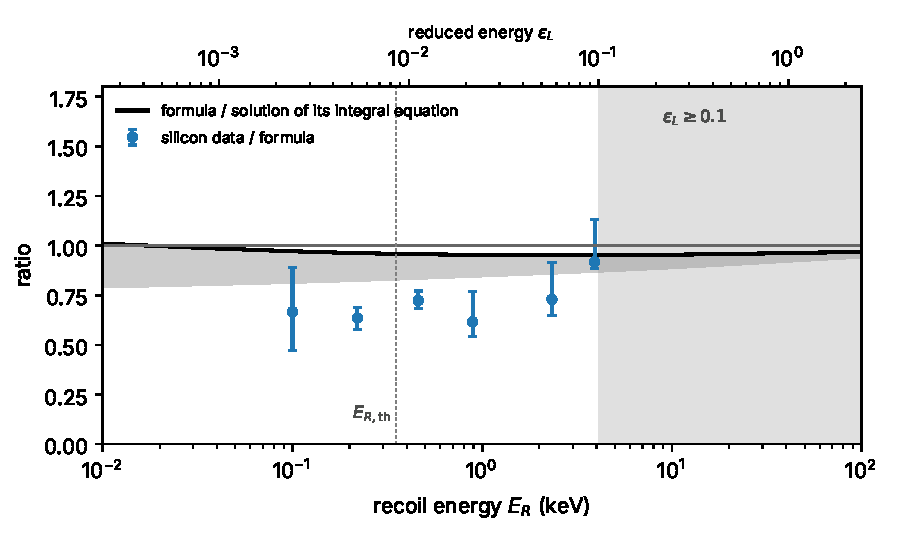
\includegraphics[width=\linewidth]{figures/ch19/limit19_3a.pdf}
\captionof{figure}{Silicon, $k_L = 0.146$, against the recoil energy. Solid: the formula divided by the numerical solution of the binary-collision equation \cref{eq:19.3-simple} with the Thomas--Fermi cross-section in the impulse approximation, continued below $x_L = 2\times10^{-3}$ as $x_L^{1/3}$; dark band: the same with continuation exponents from 1/3 to the local slope 0.363 of the computed cross-section, a sensitivity to that choice. Points: the measured silicon yields~\cite[Table~II]{albakry2023first} divided by the formula. Dashed: the constant-binding model with $U = \SI{0.15}{keV}$~\cite[Eq.~(13), Table~3]{sarkis2020study} divided by the formula. Gray: $\epsilon_L \ge 0.1$, $E_R \ge \SI{4.1}{keV}$, where the formula describes the silicon data~\cite[Sect.~II]{sarkis2020study}. Vertical line: the binary threshold $E_{R,\mathrm{th}} = \SI{352}{eV}$.}\label{fig:19-limit-lindhard}
\par}
\smallskip
Below a few keV the measured yields fall 8 to \SI{38}{\percent} under the formula, a deficit comparable to the formula's sensitivity to its softest collisions; the stored energy, the gap and the conversion to pairs that the model omits also act there.
\end{limitbox}

With the $x_L^{1/3}$ continuation the solution and the fit agree to \SI{3}{\percent} below \SI{100}{eV}, and the fit lies \SIrange{4}{5}{\percent} below the solution between 1 and \SI{20}{keV}, where $y_L$ is 0.210 against 0.220 at \SI{1}{keV}. The continuation matters more than the fit. Continuing the computed cross-section at its own local slope, 0.363 at $x_L = 2\times10^{-3}$, raises the solution by \SI{13}{\percent} at \SI{1}{keV} and by \SI{10}{\percent} at \SI{4}{keV}; an exponent of 0.30 lowers it by \SI{11}{\percent} at \SI{1}{keV}, and 0.40 raises it by \SI{40}{\percent}. The dark band of \cref{fig:19-limit-lindhard} is therefore a sensitivity to one modeling choice, not an uncertainty. Nothing places the true yield between the two continuations: below the matching point the Thomas--Fermi cross-section steepens toward $x_L^{1/2}$, while binding and the lattice remove the softest transfers altogether. Below $\epsilon_L = 2\times10^{-3}$, about \SI{80}{eV}, the whole cross-section of a slow secondary lies in the continued region, and the binary model does not determine the yield of a keV recoil there. Those are the soft collisions of the slowest secondaries, at energies of tens of eV, where atoms are bound and the binary model has least claim to hold. The equation propagates their treatment upward because every recoil ends as a population of such secondaries.

\subsection{Implicit assumptions of Lindhard quenching}\label{sec:19.3-assumptions}

Read against the partition of \cref{sec:19.1}, the chain from \cref{eq:19.3-basic} to $y_L$ makes three assumptions that its list of approximations does not name: no stored energy, electronic friction down to zero speed, and conversion to pairs in proportion. Each fails below a keV in silicon.

The first is that no energy is stored. With $U = 0$ every collision returns its full transfer to atomic motion, and an atom that ends displaced keeps no energy in the lattice: $E_{\mathrm{st}} = 0$ in \cref{eq:19.1-partition}. Restoring $U$ does not repair this. In the constant-binding model of Sarkis et al.~\cite[Eqs.~(9), (13)]{sarkis2020study} the struck atom pays $U$ before it moves, the lower limit of the integral in \cref{eq:19.3-simple} becomes $(\epsilon_Lc_LU)^{1/2}$, and the yield vanishes near $E_R = 2U$. Their fit to the silicon data above \SI{0.68}{keV} gives $U = 0.15 \pm \SI{0.06}{keV}$~\cite[Table~3]{sarkis2020study}, and with the fitted correction terms the yield reaches zero at \SI{298}{eV} (\cref{fig:19-yields}); the measured yield at \SI{100}{eV} is $0.102^{+0.034}_{-0.030}$. The later model of the same authors replaces $U$ by a function $U(E) = U_{\mathrm{FP}} + U_{\mathrm{EDFT}}(E)$: a constant $U_{\mathrm{FP}} = \SI{23.6}{eV}$, which the authors call the Frenkel-pair creation energy and take from averaged displacement thresholds, plus an energy-dependent excitation of the inner electrons. It adds electronic straggling and a modern stopping model, and it fits 102 points from \SI{0.68}{keV} to \SI{3}{MeV} with $\chi^2/\mathrm{dof} = 1870/101$; its threshold lies just above $U_{\mathrm{FP}}$~\cite[Eqs.~(2)--(4), Fig.~3]{sarkis2023ionization}. The configurational energy of a Frenkel pair in silicon is 6.8 to \SI{9.7}{eV} (\cref{sec:7.4}), a third of $U_{\mathrm{FP}}$; in the partition that part is stored energy and the rest of a threshold-sized $U_{\mathrm{FP}}$ is heat. In both models, however, the $U$ spent by secondary atoms appears as an argument of $T_{\mathrm{d}}(T_n - U)$, is missing from the damage energy, and therefore lands in the electronic share $E - T_{\mathrm{d}}$ by complement. Energy that the partition stores in defects is counted as ionization.

The second is that electronic losses follow the friction law down to zero speed. \Cref{eq:19.3-Se} gives a silicon ion of \SI{100}{eV} an electronic stopping of \SI{0.88}{eV/\angstrom}, while a binary collision at that energy cannot create a pair at all (\cref{sec:19.2-binary}), and the momentum tail lets through a fraction $5.6\times10^{-3}$ of the valence electrons (\cref{sec:19.2-soft}). Below $E_{R,\mathrm{th}}$ the friction assigns losses to final states that are strongly suppressed. The modified equation of Sarkis et al.\ also keeps a term $-\tfrac12k_L\epsilon_L^{3/2}\epsilon_{\mathrm{d}}''$, obtained from the second-order expansion with the mean nuclear transfer $\epsilon_L/2$ in a collision that also excites electrons~\cite[Eq.~(9), App.~B]{sarkis2020study}. Under approximation (D) every collision has $T_n = 0$ or $\sum_iT_{e,i} = 0$, so the cross term $T_n\sum_iT_{e,i}$ that produces it vanishes identically, and the term contradicts the separation used to obtain the stopping.

The third is that the electronic share becomes charge in proportion, $N_{\mathrm{eh}} = y_LE_R/\varepsilon_{\mathrm{eh}}$, with every pair collected and none trapped. Then $Y_q = y_L$. The excitations of a slow ion lie near the gap, where the cascade gives one pair per excitation rather than $\omega_e/\varepsilon_{\mathrm{eh}}$ (\cref{eq:19.2-charge}), so $y_L$ and $Y_q$ differ even if $y_L$ were exact. Trapping and incomplete collection lower the measured charge further (\cref{sec:18.5,sec:19.5}).

The approximations that the list does name are weakest at the same energies. The medium is a random gas of atoms, with no channels and no dependence on direction, and collisions are binary and independent, which fails in the dense cascades of germanium recoils of a few keV. The reduced energy is also convention-dependent. Sarkis et al.\ define it in their later work with the universal screening length and an effective projectile charge $Z_1 = 12$. This maps the same recoil energy to a reduced energy \SI{10}{\percent} higher than \cref{eq:19.3-reduced}~\cite[Sect.~``The nuclear recoil QF'']{sarkis2023ionization}, so that fitted constants cannot be carried from one convention to the other.

\begin{figure}[tbp]
  \centering
  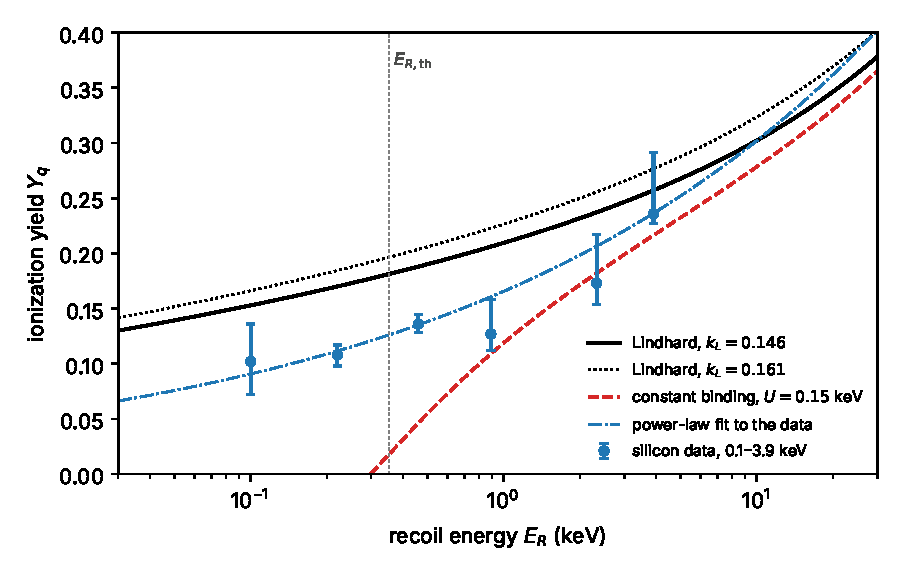
\includegraphics[width=\linewidth]{figures/ch19/fig19_3.pdf}
  \caption{Lindhard and modified-Lindhard yields of silicon against the measured ionization yield. Solid: Lindhard's formula \cref{eq:16.6-lindhard} with $k_L = 0.146$; dotted: with $k_L = 0.161$, the value of a fit of the numerical constant-binding solution to the silicon data~\cite[Table~4]{sarkis2020study}. Dashed: the constant-binding model of Sarkis et al.\ with $U = \SI{0.15}{keV}$, $C_0 = 9.1\times10^{-3}$ and $C_1 = 3.33\times10^{-5}$~\cite[Eq.~(13), Table~3]{sarkis2020study}, which vanishes at \SI{298}{eV}. Points: the silicon measurement with total uncertainties~\cite[Table~II]{albakry2023first}; dash-dotted: its power-law fit $0.302(E_R/\SI{10}{keV})^{0.261}$, pinned to the formula at \SI{10}{keV}. Vertical line: the binary threshold $E_{R,\mathrm{th}} = \SI{352}{eV}$ (\cref{sec:19.2}).}
  \label{fig:19-yields}
\end{figure}

\Cref{fig:19-yields} shows the result of these assumptions. Raising $k_L$ moves the whole curve up and away from the sub-keV data. Adding a constant binding brings the curve down to the data near \SI{2}{keV} only by introducing a cutoff that the data at 0.10 and \SI{0.22}{keV} contradict. The data themselves follow the power law $E_R^{0.26}$ from \SI{0.1}{keV} to \SI{3.9}{keV}, flatter than $y_L$ and with no threshold. Each modified model fixes one assumption and lets its fitted constants absorb the rest; a good fit therefore does not tell us which assumption was wrong. The calculation that would show it is the partition of \cref{sec:19.1} with stored energy, the excitation kernel of \cref{sec:19.2} and the cascade conversion, specified in \cref{app:E.23}. Above about \SI{4}{keV}, where stored energy and the gap are small fractions of the electronic share, Lindhard's formula describes the silicon data and needs no repair.

\subsection{Bethe stopping from the loss function}\label{sec:19.3-bethe}

At the opposite end of the speed range the stopping of an ion is a derived result. Take the dielectric stopping \cref{eq:4.4-dEdx} of a heavy projectile of charge $Z_1e$ and speed $v$ at $T = 0$, and suppose $v$ is large compared to the speeds of the electrons that hold the weight of the loss function. Split the momentum integral at a value $q_0$ chosen so that two conditions hold together: $q_0v$ lies far above the energies where $L$ has its weight, and $q_0$ is small compared to the inverse size of the atoms, so that $L(q,\omega) \simeq L(0,\omega)$ for $q < q_0$. Both are possible only if $v$ is large.

Below $q_0$ the loss function is its optical limit, and the condition $\omega \le qv$ becomes $q \ge \omega/v$. Exchanging the order of integration,
\begin{equation*}
  \int_0^{q_0}\frac{\dd q}{q}\int_0^{qv}\dd\omega\,\omega L(0,\omega) = \int_0^\infty\dd\omega\,\omega L(0,\omega)\,\ln\frac{q_0v}{\omega} ,
\end{equation*}
where the upper limit of the $\omega$ integral moved to infinity because $q_0v$ lies above the whole spectrum. Above $q_0$ the line $\omega = qv$ lies above the spectrum at every $q$ until it meets the free-electron recoil $\omega = q^2/2m_e$, at $q = 2m_ev$. Between $q_0$ and $2m_ev$ the inner integral is therefore the whole f-sum $(\pi/2)\omega_p^2$ of \cref{eq:4.4-fsumL}, and beyond $2m_ev$ it is zero, since the Bethe ridge has moved out of reach. The second piece is $(\pi/2)\omega_p^2\ln(2m_ev/q_0)$. Writing the f-sum as $\int_0^\infty\dd\omega\,\omega L(0,\omega) = (\pi/2)\omega_p^2$ in the first piece, $q_0$ cancels between the two, and with $\omega_p^2 = 4\pi\alpha\nd_e/m_e$ the prefactor $2Z_1^2\alpha/\pi v^2$ of \cref{eq:4.4-dEdx} times the f-sum $(\pi/2)\omega_p^2$ equals $4\pi Z_1^2\alpha^2\nd_e/(m_ev^2)$.

\begin{keyresult}[Bethe stopping from the loss function]
For a heavy projectile of charge $Z_1e$ and speed $v$ well above the speeds of the electrons that hold the weight of the loss function, in first order in $Z_1$,
\begin{equation}
  -\frac{\dd E}{\dd x} = \frac{4\pi Z_1^2\alpha^2\nd_e}{m_ev^2}\,\ln\frac{2m_ev^2}{\bar I} ,
  \label{eq:19.3-bethe}
\end{equation}
with the mean excitation energy defined by the logarithmic moment of the optical loss function,
\begin{equation}
  \ln\bar I = \frac{2}{\pi\omega_p^2}\int_0^\infty\dd\omega\;\omega\,L(0,\omega)\,\ln\omega ,
  \label{eq:19.3-lnI}
\end{equation}
where $\nd_e$ and $\omega_p$ count all the electrons of the target.
\end{keyresult}

\noindent This is the nonrelativistic limit of the Bethe equation of the Particle Data Group. Its bracket $\tfrac12\ln(2m_e\beta^2\gamma^2W_{\mathrm{max}}/I^2) - \beta^2$, with $W_{\mathrm{max}} = 2m_e\beta^2\gamma^2$ for a heavy projectile, becomes $\ln(2m_ev^2/I)$ up to terms of order $v^4$, and its prefactor $Kz^2(Z/A)/\beta^2$ per unit mass is $4\pi\alpha^2\nd_e/(m_ev^2)$ per unit length~\cite[Eq.~(34.5)]{navas2024review}. The Particle Data Group describes $I$ as a geometric average of the excitation energies weighted by their oscillator strengths~\cite[Sect.~34.2.1]{navas2024review}; \cref{eq:19.3-lnI} makes the weight precise for a condensed medium. It is the loss function, not $\varepsilon_2$, because the projectile couples to the total potential, and the logarithm sits inside the f-sum weight $\omega L$. The prefactor of \cref{eq:19.3-bethe} depends on the electron density alone, as \cref{sec:4.4} anticipated; the solid enters only through $\bar I$, and only logarithmically.

\begin{workedexample}{The mean excitation energy of silicon}\label{we:19-lnI}
Start with the four valence electrons in the single damped oscillator of \cref{we:4-oscillatorL} at $q \to 0$: $L(0,\omega) = \omega_p^2\varGamma_{\mathrm{w}}\omega/[(\omega^2 - \bar E^2)^2 + \varGamma_{\mathrm{w}}^2\omega^2]$ with $\omega_p = \SI{16.6}{eV}$, $\bar E = \SI{17.4}{eV}$ and $\varGamma_{\mathrm{w}} = \SI{3.66}{eV}$. For a narrow line \cref{eq:19.3-lnI} would give $\bar I = \bar E$, since all the weight sits at one energy. The damping spreads it: the model puts \SI{88}{\percent} of its f-sum between 10 and \SI{30}{eV}, but \SI{7.8}{\percent} between 30 and \SI{100}{eV} and \SI{2.4}{\percent} above, in a tail $\omega L \propto \varGamma_{\mathrm{w}}\omega_p^2/\omega^2$ that the logarithm weights heavily. Numerically,
\begin{equation*}
  \ln\bar I_{\mathrm{val}} = \frac{2}{\pi\omega_p^2}\int_0^\infty\dd\omega\,\omega L(0,\omega)\ln\frac{\omega}{\SI{1}{eV}} = 3.012 , \qquad \bar I_{\mathrm{val}} = \SI{20.3}{eV} ,
\end{equation*}
\SI{17}{\percent} above $\bar E$; a damping of \SI{2}{eV} brings it to \SI{19.0}{eV}. The inverse moment of \cref{eq:4.4-inverse} fixed $\bar E$ from the low-energy side of the spectrum; $\bar I$ is set by the high-energy side, and the two mean energies agree only for a narrow line.

The valence electrons are four of fourteen, and the core changes the answer by an order of magnitude. Take the measured loss function of \cref{sec:10.7}, which extends to \SI{30}{keV}. For all fourteen electrons $\omega_p = \SI{31.05}{eV}$ and $(\pi/2)\omega_p^2 = \SI{1514}{eV^2}$; the tabulated spectrum holds \SI{1537}{eV^2}, \SI{1.5}{\percent} more. Split at \SI{90}{eV}, below the L edge, and at \SI{1.83}{keV}, below the K edge, the f-sum weight $w_j$ and the logarithmic mean energy $\omega_j$ of each band are
\begin{equation*}
  \text{valence: } 0.280,\ \SI{19.5}{eV} ; \qquad \text{L shell: } 0.607,\ \SI{246}{eV} ; \qquad \text{K shell: } 0.113,\ \SI{3.17}{keV} ,
\end{equation*}
so that, with the spectrum normalized to its own f-sum, $\ln(\bar I/\SI{1}{eV}) = \sum_jw_j\ln(\omega_j/\SI{1}{eV}) = 0.832 + 3.340 + 0.910 = 5.082$ and $\bar I = \SI{161}{eV}$. Rescaling the spectrum to the exact f-sum leaves this value unchanged. It lies \SI{7}{\percent} below the adopted \SI{173.0}{eV} of the Particle Data Group~\cite{pdg2024atomic}, and the \SI{1.5}{\percent} excess of the tabulated f-sum is a measure of the error of the data. The L shell holds \SI{61}{\percent} of the oscillator strength and the valence electrons, which set every dark-matter rate of \cref{chap:10}, \SI{28}{\percent}; without the core shells $\bar I$ would be the \SI{19.5}{eV} of the valence band.
\end{workedexample}

The derivation needs two conditions, and both fail for recoils. The split at $q_0$ requires $2m_ev^2 \gg \bar I$, so that the logarithm is large: a proton of \SI{1}{MeV} has $2m_ev^2 = \SI{2.2}{keV}$, thirteen times the $\bar I$ of silicon, while a silicon recoil of \SI{10}{keV} has \SI{0.78}{eV}, $4.5\times10^{-3}$ of it, and \cref{eq:19.3-bethe} would give a negative stopping. The first-order treatment requires $Z_1\alpha/v \ll 1$: 0.16 for the proton, 117 for the recoil. \Cref{lim:19.3b} shows the first condition in an electron gas, where both formulas can be evaluated exactly.

\begin{limitbox}[Bethe stopping][lim:19.3b]
The Bethe formula in its nonrelativistic limit~\cite[Eq.~(34.5)]{navas2024review}, \cref{eq:19.3-bethe}: $-\dd E/\dd x = (4\pi Z_1^2\alpha^2\nd_e/m_ev^2)\ln(2m_ev^2/\bar I)$, with $\bar I$ from \cref{eq:19.3-lnI}.
\par\smallskip
{\centering
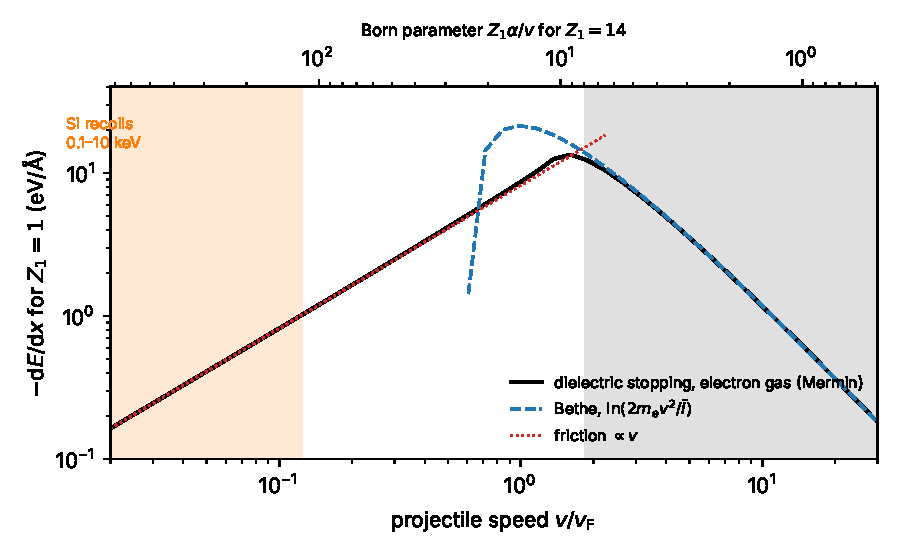
\includegraphics[width=\linewidth]{figures/ch19/limit19_3b.pdf}
\captionof{figure}{Stopping of a heavy projectile with $Z_1 = 1$ in the electron gas of the silicon valence density ($k_{\mathrm{F}} = \SI{1.8085}{\angstrom^{-1}}$, $v_{\mathrm{F}} = 6.98\times10^{-3}$, $\omega_p = \SI{16.6}{eV}$), against its speed. Solid: the dielectric stopping \cref{eq:4.4-dEdx} with the Mermin dielectric function of \cref{sec:4.5} and relaxation rate $0.1\,\omega_p$, a modeling choice that keeps the f-sum. Dashed: \cref{eq:19.3-bethe} with the model's own $\bar I = \SI{17.9}{eV}$ from \cref{eq:19.3-lnI}. Dotted: the friction law, linear in $v$, fitted at the lowest speed. Gray: $v \ge 1.84\,v_{\mathrm{F}}$, where the Bethe formula lies within \SI{10}{\percent} of the dielectric stopping. Orange: the speeds of silicon recoils from 0.1 to \SI{10}{keV}. Top axis: the Born parameter $Z_1\alpha/v$ of a silicon ion, $Z_1 = 14$.}\label{fig:19-limit-bethe}
\par}
\smallskip
Below about $2v_{\mathrm{F}}$ the momentum transfers that reach the loss function no longer exhaust its f-sum, and the stopping turns over into the friction regime, where it is set by the low-energy side of $L$ and not by $\bar I$.
\end{limitbox}

The approach to the Bethe form is fast once it starts: the dielectric stopping lies within \SI{5}{\percent} of \cref{eq:19.3-bethe} above $2.27\,v_{\mathrm{F}}$ and within \SI{1}{\percent} above $4.3\,v_{\mathrm{F}}$. The Bethe logarithm vanishes at $v = (\bar I/2m_e)^{1/2} = 0.60\,v_{\mathrm{F}}$, below which the formula has no meaning. In the friction regime the same Mermin electron gas gives a stopping of \SI{1173}{eV/\angstrom} times $v$ for $Z_1 = 1$, constant to \SI{0.1}{\percent} up to $v = 0.1\,v_{\mathrm{F}}$. Silicon recoils, at 0.013 to $0.13\,v_{\mathrm{F}}$, sit deep in that regime, with Born parameters from 117 to over a thousand. The corrections that the Particle Data Group lists for slower projectiles, shell corrections, the Barkas term of order $Z_1^3$ and the Bloch term, extend the Bethe formula down to about $\beta \approx 0.05$, and between $\beta = 0.01$ and 0.05 no theory is satisfactory~\cite[Sect.~34.2.6]{navas2024review}. Recoils from dark matter move at $\beta < 10^{-3}$. Computing $L(q,\omega)$ to the core energies that set $\bar I$, with local fields and the core states of \cref{app:E.15}, is the task of \cref{app:E.6,app:E.16}; for slow ions it fixes the first-order stopping of \cref{sec:19.2-soft}, not the yield.

A fast heavy ion, by contrast, leaves a track of $10^2$ to $10^4$ correlated collisions in a lattice already disturbed by the previous ones, and what a track detector reads is a defect configuration, not an excitation spectrum; damage-track and paleo-detector searches need \cref{eq:19.3-bethe,eq:19.3-Se} as input to a transport calculation of that track.
